\documentclass[12pt]{article}

\usepackage{geometry}
\usepackage[utf8]{inputenc}
\usepackage[T2A]{fontenc}
\usepackage[russian]{babel}
\usepackage{graphicx}
\usepackage{caption}
\usepackage{amssymb, gensymb, amsmath}
\usepackage{mathrsfs}
\usepackage{array, colortbl}
\usepackage{multicol}

\title{{\bf Лабораторная работа 4.\, 2. \\ Исследование энергетического спектра $\beta$-частиц и определение их максимальной энергии при помощи магнитного спектрометра}}
\author{Лось Денис (группа 618)}
\date{23 ноября 2018}

\begin{document}

\maketitle

\paragraph*{Цель работы: } с помощью магнитного спектрометра исследовать энергетический спектр $\beta$-частиц при распаде ядер цезия и определить их максимальную энергию. Калибровка спектрометра осуществляется по энергиеям электронов внутренней конверсии цезия.

\section*{Введение в теоритическую часть}
\par
	Энергетический спектр $\beta$-частиц в нерелятивистком случае
\[
	\frac{dN}{dE} \approx \sqrt{E} \cdot (E_e - E)^2
\]
\par
	Связь между числом частиц, регистрируемой установкой, и функцией $W(p_e) = dW / dp_e$
\[
	N(p_e) \approx W(p_e) \Delta p_e
\]
\par
	Ширина интервала, регистрируемая спектрометром
\[
	\Delta p_e = \frac{1}{2} \frac{\Delta f}{f} p_e
\]
\par
	Так как $\Delta f / 2f$ определяется геометрией установки и потому постоянно, получим в итоге
\[
	N(p_e) = CW(p_e) \cdot p_e \quad (C = const)
\]
\par
	График Ферми-Кюри
\[
	\frac{\sqrt{N(p)}}{p} \approx E_e - E.
\]

\section*{Ход работы и результаты исследования}
\par
	Измерения фона:
\begin{table}[h!]
	\centering
	\begin{tabular}{|c|c|c|c|}
	\hline
		$t$, c & $N_\text{ф}$, 1/c & $\Delta N_\text{ф}$, 1/c & $\varepsilon$, \% \\
	\hline
		100 & 2.3094 & 0.152 & 6.5 \\
	\hline
		600 & 2.4349 & 0.064 & 2.8 \\ 
	\hline
	\end{tabular}
\end{table}
\par
	График зависимости интенсивности от тока магнитной линзы
\begin{figure}[h!]
	\centering
	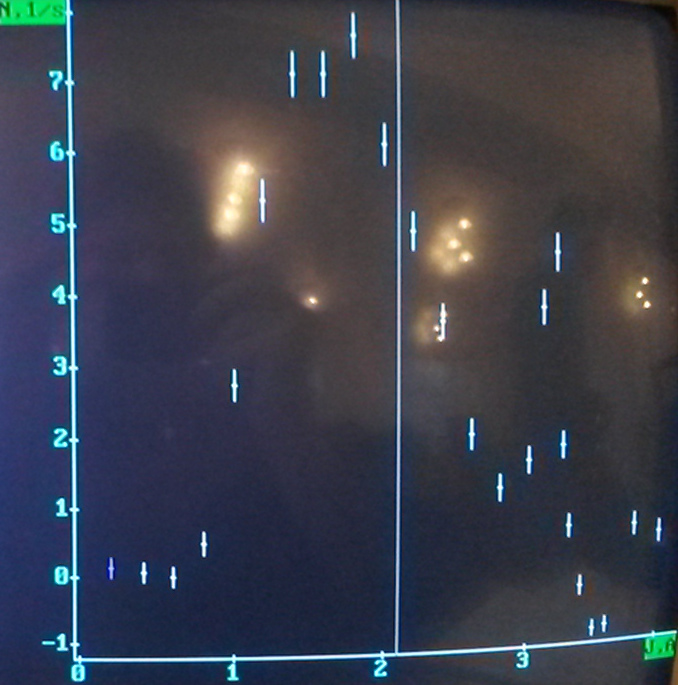
\includegraphics[width = 12cm, height = 10cm]{first_graph.jpg}
\end{figure}
\newpage
\par
	График Ферми-Кюри:
\begin{figure}[h!]
	\centering
	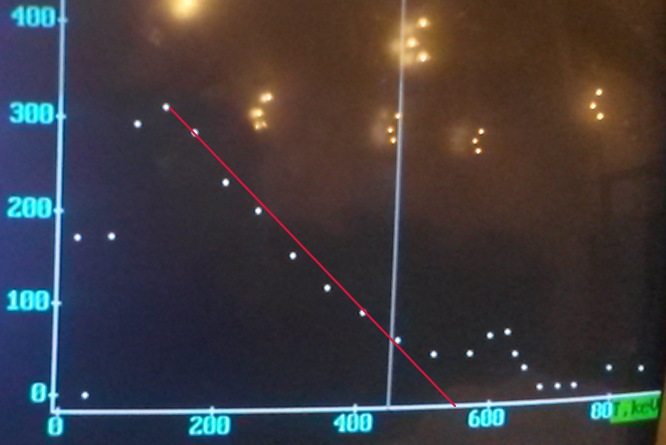
\includegraphics[width = 12cm, height = 10cm]{energy.png}
\end{figure}
\par
	Максимальная энергия в $\beta$-спектре
\[
	E_\text{max} = \left(560 \pm 20\right) \, \text{кэВ}
\]
\newpage
\par
	Результаты измерений
\begin{figure}[h!]
	\centering
	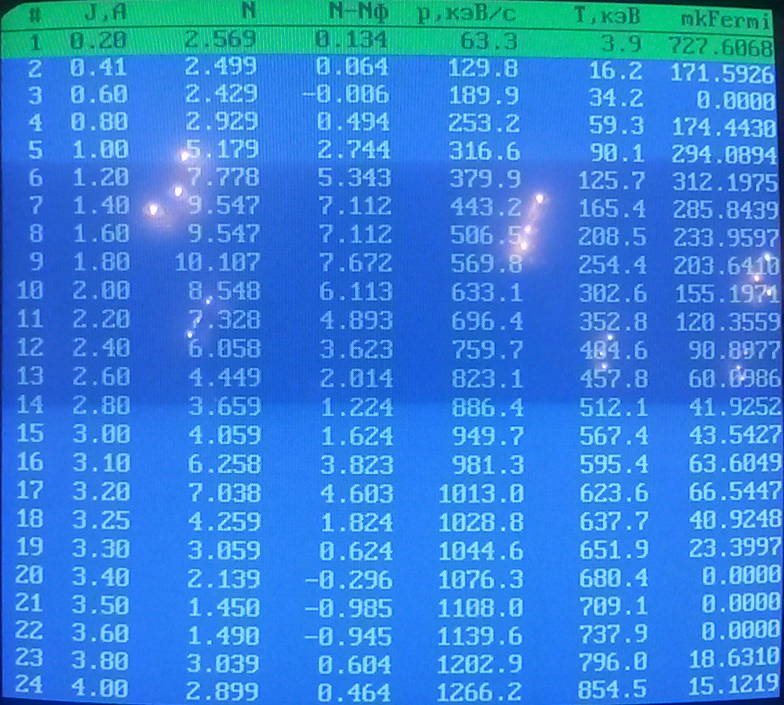
\includegraphics[width = 12cm, height = 10cm]{results.png}
\end{figure}

\end{document}